\subsubsection{Aufführungspraktische Bedingungen}

\hypertarget{RefHeadingToc100333744}{}Die Besetzung einer bestimmten
Komposition oder eines bestimmtes Arrangements spiegelt die
aufführungspraktischen Bedingungen wider, die in Ruhmannsfelden zur
Entstehungszeitpunkt des entsprechenden Werks herrschten. Aus dem
Werkverzeichnis lassen sich darüber hinaus Veränderungen ablesen, die
sich im Laufe der Zeit an den aufführungspraktischen Verhältnissen in
Ruhmannsfelden ergeben haben, und mit den Wissen um die Besetzung aus
Dokumenten und Interviews vergleichen und konkretisieren.

Wie aus dem Werkverzeichnis ersichtlich ist, begleitet in den frühen
Werken (z. B. Adjuva nos Es-Dur op. 8, „Mater-Dei“-Messe F-Dur op. 16)
ein Streichorchester Chor und Orgel, in den späten Werken (z. B. Ecce
sacerdos F-Dur op. 57, Juravit Dominus B-Dur op. 58) übernimmt diese
Funktion ein Blechbläserquartett. Nur ganz selten ist das
Blechbläserquartett in einem frühen Werk (z. B. „Laurentius“-Messe
C-Dur op. 14) besetzt. Wie ein Blick auf die entsprechenden Autographen
verrät, hat Högn das Blechbläserquartett in allen frühen Werken
nachträglich hinzugefügt.

Aus den Autographen geht ebenso hervor, dass Högn eine
Streicherbesetzung zur Verfügung stand, in der alle Instrumente der
Familie der Streichinstrumente vertreten waren, auch die seltener
gespielten Instrumente Bratsche und Kontrabass. Das Orchestermaterial
von Högns Vorgänger Max Weig macht hingegen deutlich, dass Weig noch
keine vollständige Streicherbesetzung einsetzen konnte. Ein
vollständiges Streichorchester als Begleitung des Kirchenchores an
Festtagen ist deshalb eine Erscheinung, die erst in der ersten Hälfte
des 20. Jahrhunderts auftritt. Ein möglicher Gründ für das erstarkende
Streichorchester liegt im überdurchschnittlich großen
Bevölkerungszuwachs Anfang des 20. Jahrhundert in Ruhmannsfelden.
Zwischen 1870 und 1920 wuchs die Ruhmannsfeldener Bevölkerung um fast
fünfzig Prozent auf knapp 1500 Einwohner an. \footnote{Bayerisches
Landsamt für Statistik} Die Zahl der in Ruhmannsfelden tätigen Lehrer
erhöhte sich deshalb von vier auf sieben. Alle Lehrer waren aufgrund
der intensiven musikalischen Lehrerausbildung im Streichorchester
einsetzbar. Parallel zur ansteigenden Bevölkerungsanzahl stieg auch die
Zahl an Ärzten und Apothekern, die meist während ihrer gymnasialen
Ausbildung das Spielen eines Streichinstruments erlernten. So wirkten
im Orchester Högns namentlich bekannt der Tierarzt Dr. Haug
(Violoncello), \footnote{Interview Nr. 13, Lorenz Schlagintweit,
29.11.2003; Absatz 6} der Apotheker Vitus Voit (Violine),\footnote{
Interview Nr. 13, Lorenz Schlagintweit, 29.11.2003; Absatz 2} der Sohn
des Arztes Dr. Danziger, Franz Danziger (Violine), späterer
Kirchenchorleiter und Högns Nachfolger mit.


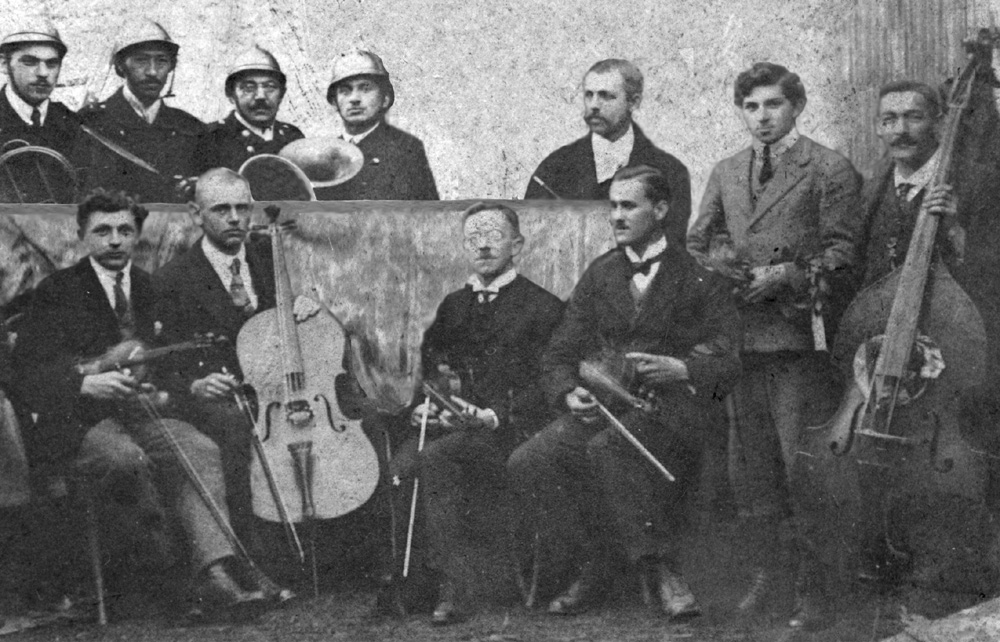
\includegraphics[width=15.822cm,height=10.109cm]{pictures/zulassungsarbeit-img072.jpg}


Abb. \stepcounter{Abb}{\theAbb}: Turnverein-Orchester bei den
„Holledauer Fidel“-Aufführungen 1923 (montiert aus dem großen
Gruppenfoto); sitzend v. l: Ludwig Rauscher, Dr. Haug, Vitus Voit;
stehend, 2. v. l. Josef Baumann, 3. v. l. Michael Wurzer, 5. v. l.
August Högn, 6. v. l. Max Rauscher

Auf dem Foto, das anlässlich der Aufführungen des „Holledauer Fidels“
1923 aufgenommen wurde, ist zu erkennen, dass die Streicher auch
gelegentlich von Blechbläsern unterstützt wurden. Eine
\zitat{„großes Orchester aus lauter Ruhmannsfeldener
Musiker“}  \footnote{Dokument Nr. 98, Geschichtliches über die Erbauung
der Turnhalle in Ruhmannsfelden, 1928} soll laut einem Artikel aus der
Turnvereins-Chronik die Einweihungsfeier der Turnhalle 1928 feierlich
umrahmt haben. Sicherlich wurden hier neben Streichinstrumenten auch
Blasinstrumente eingesetzt. In den geistlichen Kompositionen von Högn
ist aber eine gleichzeitige Besetzung aus beiden Instrumentengruppen
äußerst selten, obwohl ihm während seines gesamten Wirkens in
Ruhmannsfelden Musiker aus den Blaskapellen in Ruhmannsfelden,
beispielsweise aus der Blaskapelle Wiesinger (Abb. 72), zur Verfügung
gestanden sind. Der Grund hierfür liegt in der kleinen Orgelempore in
Ruhmannsfelden, die lediglich einem kleinen Landchor ausreichend Platz
bot. Ein Chor und ein Streichquintett mit sperrigem Kontrabass hatten
hier enorme Platzprobleme.

Der Ausbruch des 2. Weltkrieges stellt für die Streichorchestertradition
in Ruhmannsfelden einen scharfen Einschnitt dar. Die Lehrer Gruber,
Schultz, Friedrich und Kestlmeier, die alle auch als Beteiligte an der
Kirchenmusik genannt wurden, wurden 1939 zum Kriegsdienst
eingezogen. \footnote{Reicheneder-Chronik, Schulwesen, Blatt 112
Vorder- und Rückseite} Ein weiterer Grund, der zum Niedergang des
Streichorchesters beitrug und den Übergang zum Bläserquartett notwendig
machte, war die radikalen Einschränkungen in der Lehrerausbildung durch
die Reform im Jahr 1935. \footnote{Goller, Seite 15}

\begin{flushleft}
\tablefirsthead{}
\tablehead{}
\tabletail{}
\tablelasttail{}
\begin{supertabular}{m{7.573cm}m{8.08cm}}

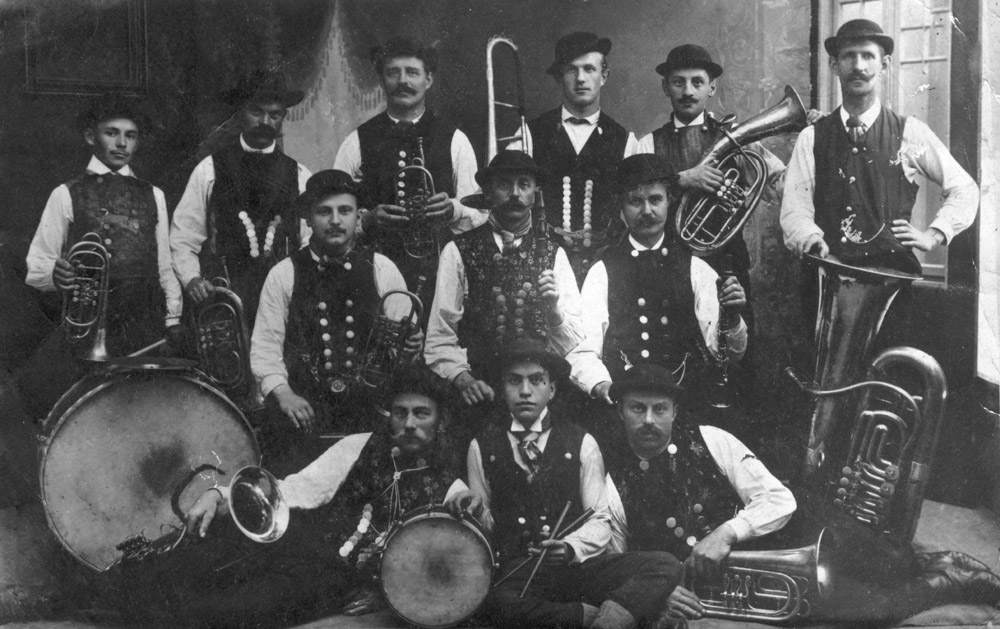
\includegraphics[width=7.391cm,height=4.703cm]{pictures/zulassungsarbeit-img073.jpg}

\label{bkm:Ref100229810}Abb. \stepcounter{Abb}{\theAbb}: Blaskapelle
Wiesinger, obere Reihe 3. v. r. Rudolf Schwannberger, 2. v. r. Michael
Wurzer, 1 v. r. Josef Baumann &

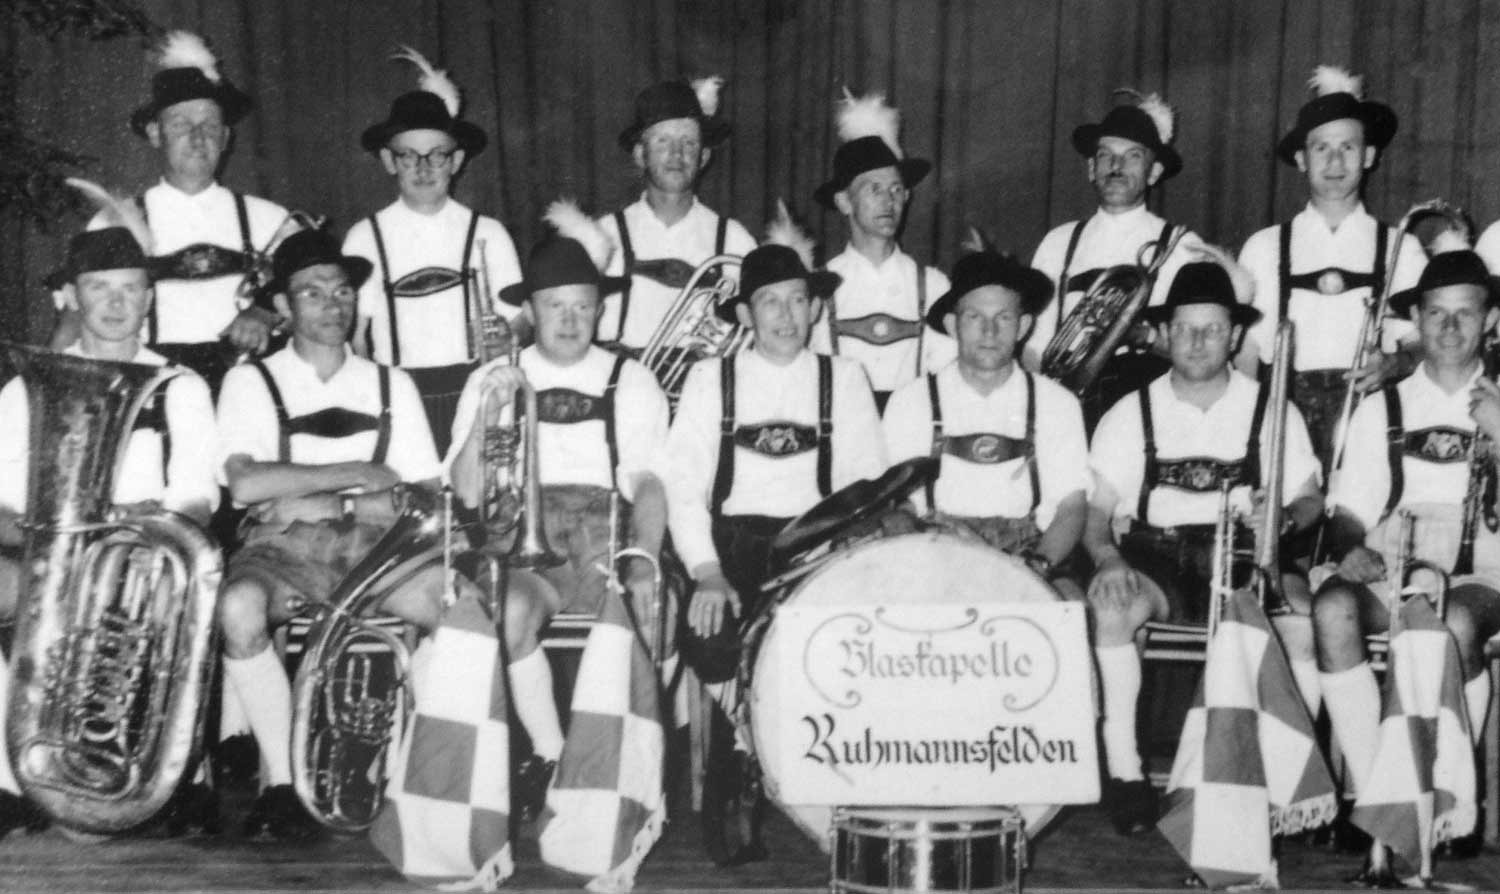
\includegraphics[width=7.897cm,height=4.706cm]{pictures/zulassungsarbeit-img074.jpg}

\label{bkm:Ref100229831}Abb. \stepcounter{Abb}{\theAbb}:
Ruhmannsfeldener Blaskapelle (untere Reihe 2. v. l. Lorenz
Schlagintweit)\\
\end{supertabular}
\end{flushleft}
War der Einsatz des Blechbläserquartetts zu Beginn des 2. Weltkrieges
noch aus der Not geboren, so machen Högns Kompositionen, die in der
Nachkriegszeit entstanden sind, und die vielen Arrangements, in denen
er das Bläserquartett hinzugefügt hat, den Eindruck, dass Högn Gefallen
an dem Quartett gefunden hatte und gar nicht mehr daran dachte, an die
Streichorchestertradition anzuknüpfen. Die „Ruhmannsfeldener
Blaskapelle“ (Abb. 73) war ein Ensemble, in dem sich kurz nach dem
Krieg ehemalige Militärmusiker, vertriebene Profimusiker und gute
Amateure zu einer hervorragenden und durch zahlreiche Rundfunkaufnahmen
ausgezeichneten Bläserformation zusammenfanden. Aus diesem Ensemble
ließ sich für den Einsatz in der Kirchenmusik ein höchst
leistungsfähiges Quartett ausgliedern, dessen Qualität das
Streichorchester auch zu seinen besten Zeiten bei weitem nicht erreicht
hätte. \footnote{Interview Nr. 13, Lorenz Schlagintweit, 29.11.2003,
Absatz 8, 12}

\begin{flushleft}
\tablefirsthead{}
\tablehead{}
\tabletail{}
\tablelasttail{}
\begin{supertabular}{m{6.019cm}}

\begin{center}

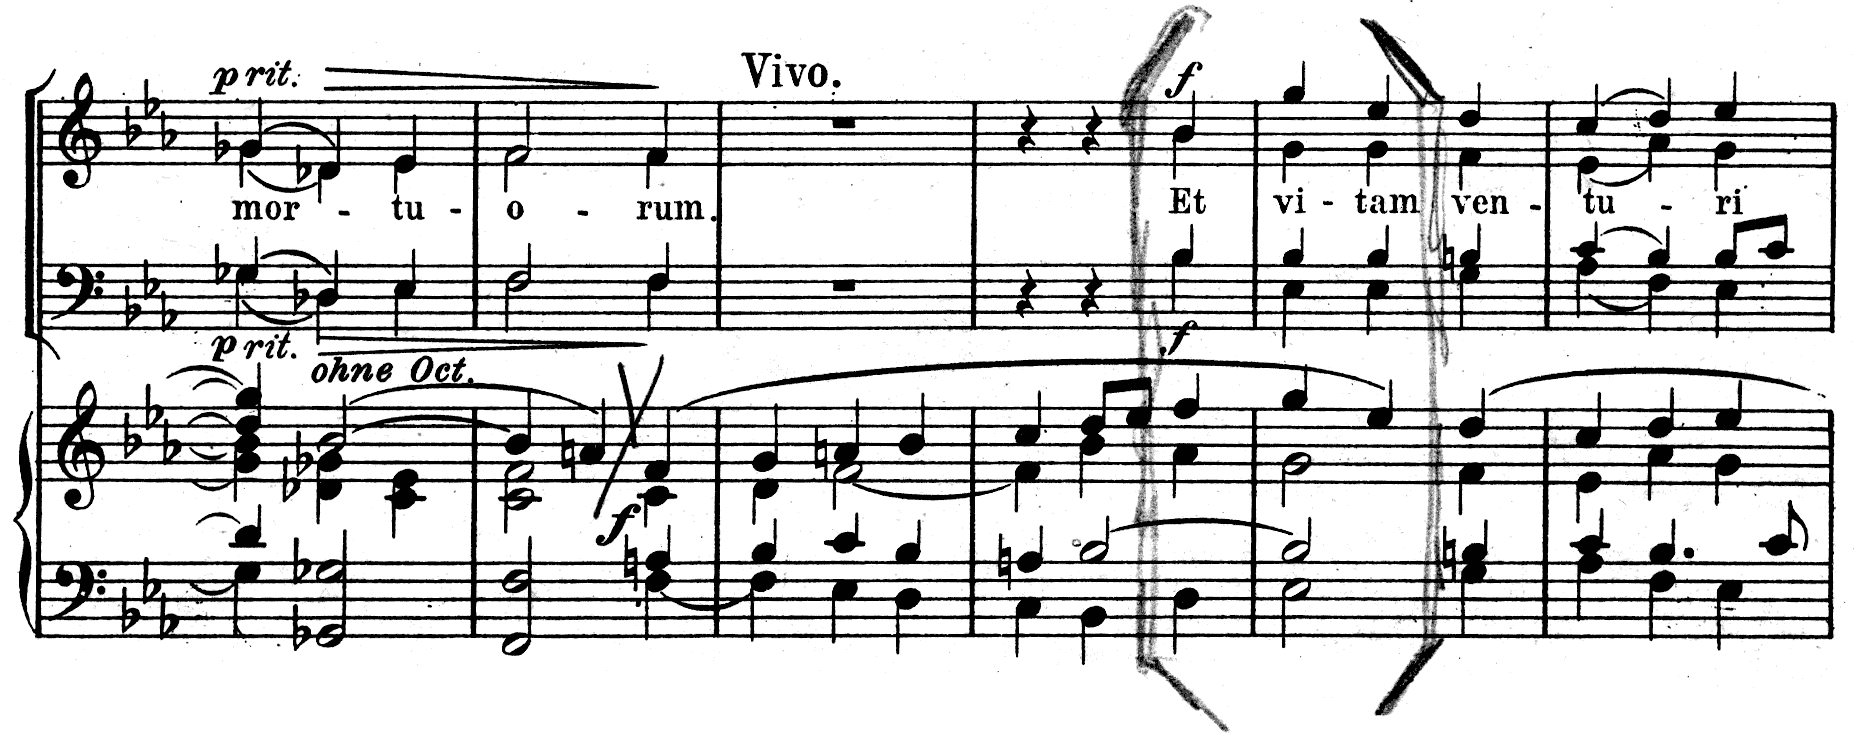
\includegraphics[width=5.837cm,height=2.35cm]{pictures/zulassungsarbeit-img075.png}

\end{center}
Abb. \stepcounter{Abb}{\theAbb}: „Loreto“-Messe von Vinzenz Goller,
Credo\\
\end{supertabular}
\end{flushleft}
Darüber hinaus war der Aufwand, Stimmen für ein Bläserquartett zu
schreiben, wesentlich geringer, als Notenmaterial für ein
Streichquintett anzufertigen. Im Gegensatz zum Streichorchester, das
nur bei „a-capella“-Stellen pausierte, beschränkte sich die Beteiligung
des Bläserquartetts auf kürzere und sehr effektvolle Einwürfe. Das
„colla-parte“-Spiel der Blechblasinstrumente deutete Högn in seinen
handschriftlichen Partituren und ebenso in den gedruckten Partituren,
die er arrangierte, durch eine Einrahmung der entsprechenden Stellen
mit Balken an und ersparte sich so die Anfertigung neuer Partituren
oder das Hinzufügen weiter Systeme. Der Einsatz des Bläserquartetts
durch Högn hatte auch durchaus seine Vorbilder. Als Prototyp für diese
Instrumentationstechnik kann wohl die „Loreto“-Messe von Vinzenz Goller
angesehen werden. Auch in dieser Partitur erscheinen für das
Bläserquartett keine Noten. Högn hat die entsprechenden Stellen, an
denen das Bläserquartett spielt, mit Balken versehen.

An der Besetzung der 13 Marienlieder tritt die Entwicklung des Chores
und die Verfügbarkeit brauchbarer Stimmen für den solistischen Gesang
während der drei Dienstzeiten von Högn als Chorregent deutlich zu Tage
wie bei sonst keinem Genre in Högns Werk. Die Besetzung der
Marienlieder ändert sich im Laufe der 13 Nummern von einer
Chorbesetzung ohne Solopart, über eine Chorbesetzung mit immer
wichtiger werdendem Solopart, schließlich zu Solo-Liedern ohne Chor.
Somit lässt sich die Entwicklung von einem Chor normaler Größe zu
Beginn von Högns Chorleitertätigkeit zu einem aus drei Fraustimmen
bestehenden „Chor“ am Ende seiner Dienstzeit erkennen. Das Marienlied
Nr. 12 op. 63, Högns letztes Werk während seiner Chorregentenzeit, ist
größtenteils zweistimmig solistisch und nur in den letzten vier Takten
dreistimmig besetzt, sodass auch neben den Sängerinnen Mathilde
Glasschröder und Barbara Essigmann die als schlechte Alt-Sängerin
bekannte Theres Raster kurz zum Einsatz kam. Die späteren Marienlieder
mit Sopran-Solo sind der außergewöhnlichen sängerischen
Naturbegabung, \footnote{Interview Nr. 13, Lorenz Schlagintweit,
29.11.2003, Absatz 2} der Sopranistin Mathilde Glasschröder (Abb. 75)
auf dem Leib geschrieben. Das Bass-Solo des Marienlieds Nr. 11 sang der
als voll tönende Bass \footnote{Interview Nr. 18, Centa Schwannberger,
14.9.2004, Absatz 10} geltende Rudolf Schwannberger (Abb. 76). Das –
nach der Opus-Zahl zu urteilen – während des 2. Weltkrieg entstandene
Marienlied Nr. 6 F-Dur op. 41 trägt mit seiner vierstimmigen
Frauenchorbesetzung dem Mangel an Männerstimmen Rechnung.

\begin{center}
\begin{minipage}{9.096cm}
\begin{flushleft}
\tablefirsthead{}
\tablehead{}
\tabletail{}
\tablelasttail{}
\begin{supertabular}{m{4.335cm}m{4.361cm}}

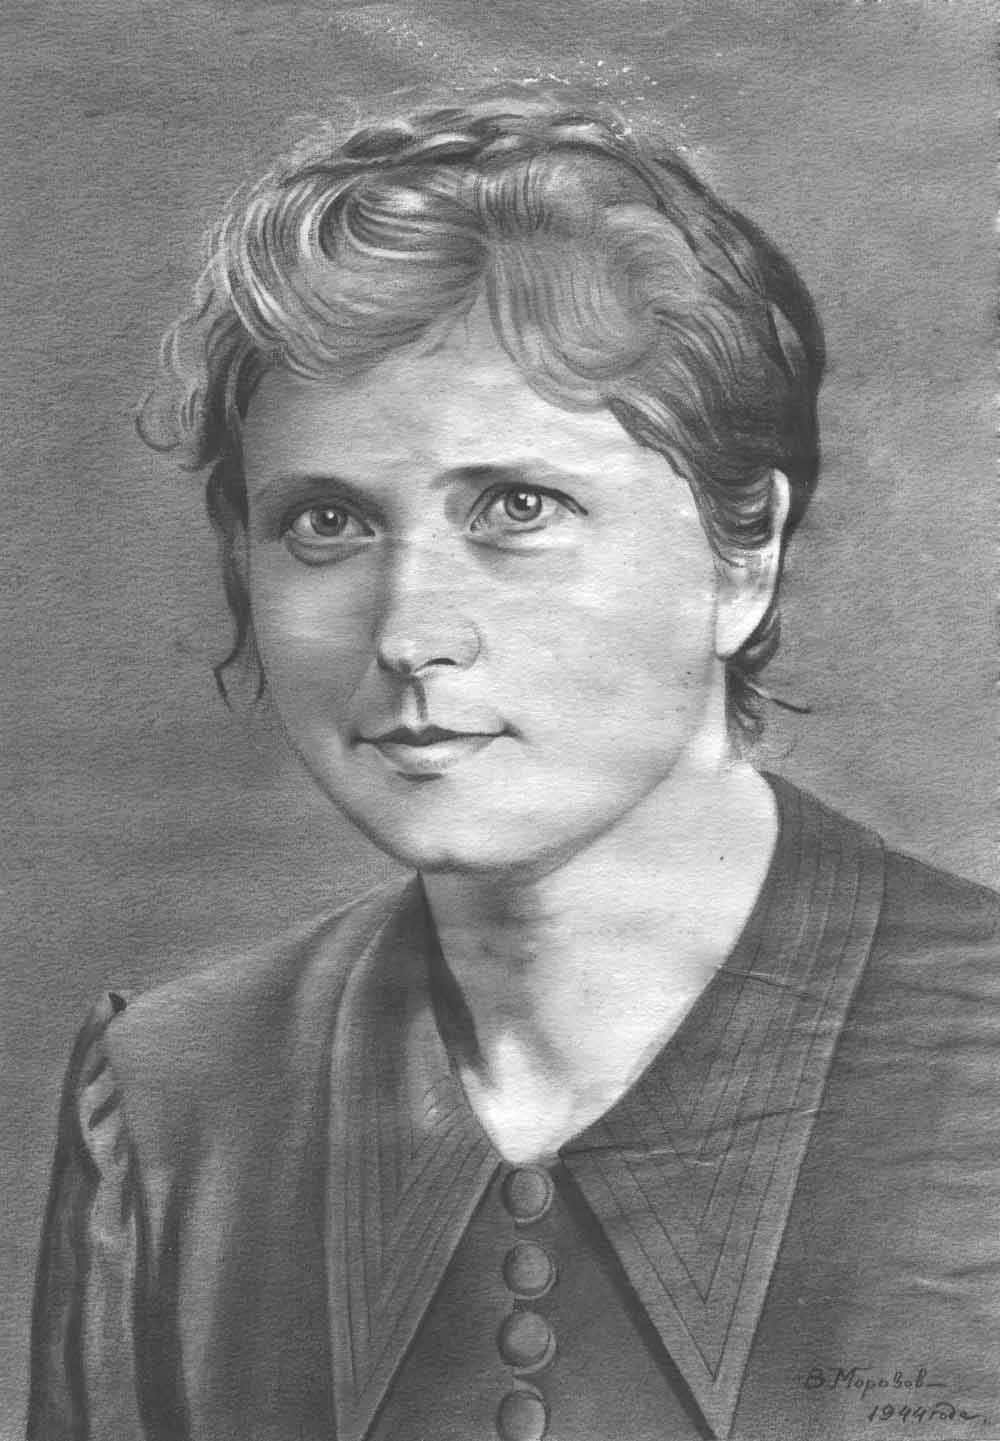
\includegraphics[width=4.154cm,height=5.985cm]{pictures/zulassungsarbeit-img076.jpg}

\label{bkm:Ref100231023}Abb. \stepcounter{Abb}{\theAbb}: Mathilde
Glaschröder &

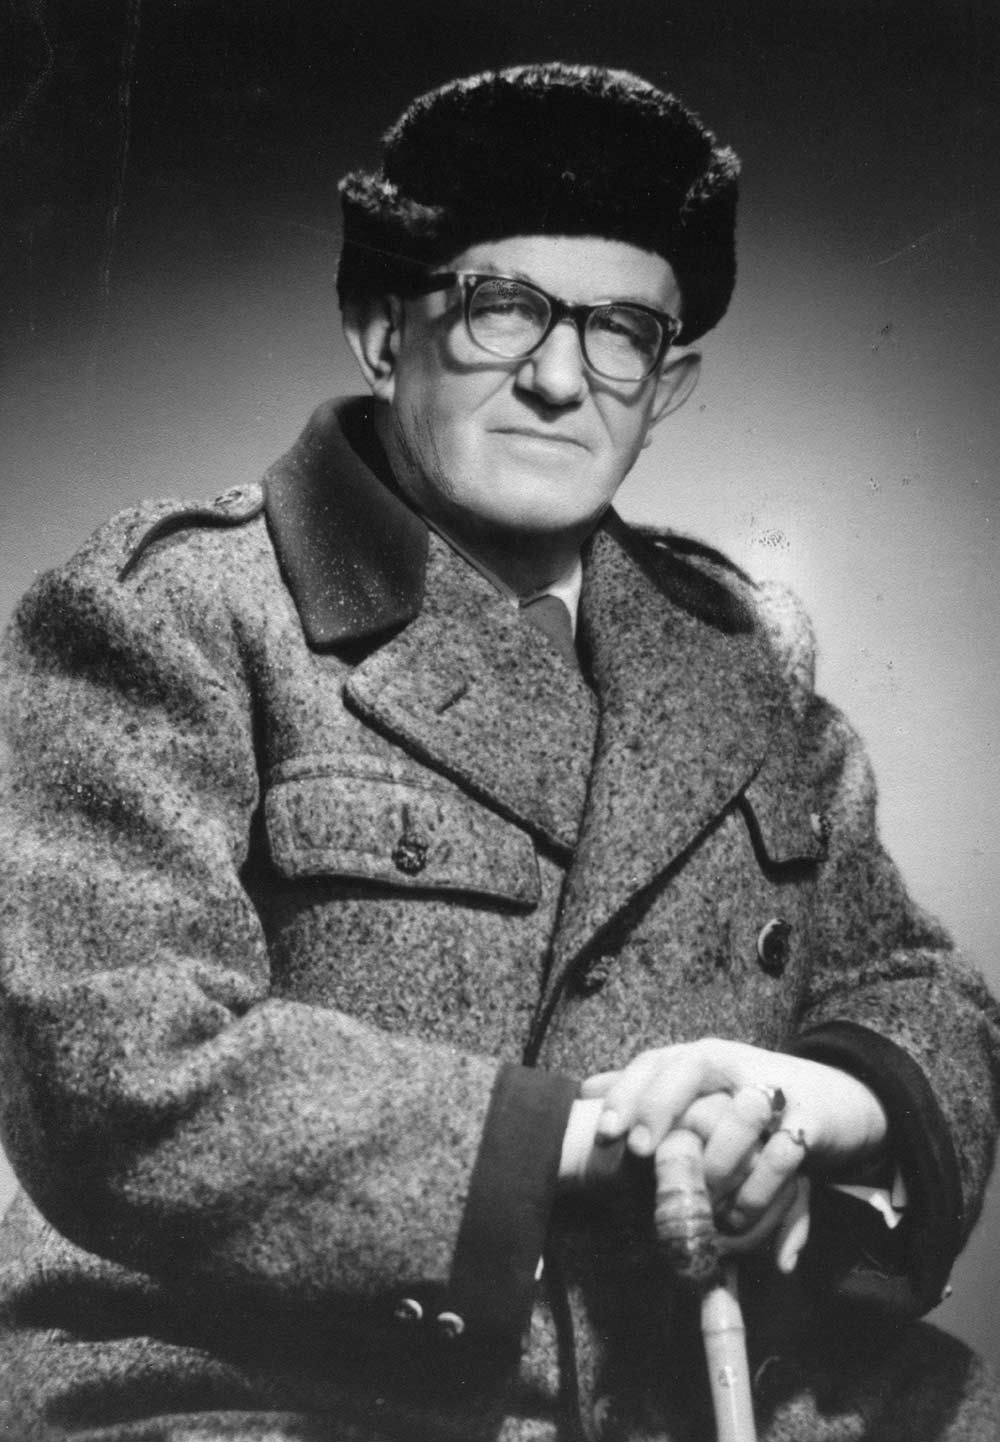
\includegraphics[width=4.18cm,height=5.988cm]{pictures/zulassungsarbeit-img077.jpg}

\label{bkm:Ref100234796}Abb. \stepcounter{Abb}{\theAbb}: Rudolf
Schwannberger\\
\end{supertabular}
\end{flushleft}
\end{minipage}
\end{center}


